%%%%%%%%%%%%%%%%%%%%%%%%%%%%%%%%%%%%%%%%%%%%%%%%%%%%%%%%%%%%%%%%%%%%%%%%
%    INSTITUTE OF PHYSICS PUBLISHING                                   %
%                                                                      %
%   `Preparing an article for publication in an Institute of Physics   %
%    Publishing journal using LaTeX'                                   %
%                                                                      %
%    LaTeX source code `ioplau2e.tex' used to generate `author         %
%    guidelines', the documentation explaining and demonstrating use   %
%    of the Institute of Physics Publishing LaTeX preprint files       %
%    `iopart.cls, iopart12.clo and iopart10.clo'.                      %
%                                                                      %
%    `ioplau2e.tex' itself uses LaTeX with `iopart.cls'                %
%                                                                      %
%%%%%%%%%%%%%%%%%%%%%%%%%%%%%%%%%%
%
%
% First we have a character check
%
% ! exclamation mark    " double quote  
% # hash                ` opening quote (grave)
% & ampersand           ' closing quote (acute)
% $ dollar              % percent       
% ( open parenthesis    ) close paren.  
% - hyphen              = equals sign
% | vertical bar        ~ tilde         
% @ at sign             _ underscore
% { open curly brace    } close curly   
% [ open square         ] close square bracket
% + plus sign           ; semi-colon    
% * asterisk            : colon
% < open angle bracket  > close angle   
% , comma               . full stop
% ? question mark       / forward slash 
% \ backslash           ^ circumflex
%
% ABCDEFGHIJKLMNOPQRSTUVWXYZ 
% abcdefghijklmnopqrstuvwxyz 
% 1234567890
%
%%%%%%%%%%%%%%%%%%%%%%%%%%%%%%%%%%%%%%%%%%%%%%%%%%%%%%%%%%%%%%%%%%%
%
\documentclass[12pt]{iopart}
% \newcommand{\gguide}{{\it Preparing graphics for IOP Publishing journals}}
%Uncomment next line if AMS fonts required
%\usepackage{iopams}

% hyperref makes references clicky. use \url{www.example.com} or \href{www.example.com}{description} to add a clicky url
\usepackage{nameref,hyperref}

% use "section" label for sections, subsections and subsubsections with the `autoref` command
% https://tex.stackexchange.com/questions/177007/autoref-showing-subsection-and-subsubsection
\let\subsectionautorefname\sectionautorefname
\let\subsubsectionautorefname\sectionautorefname


% for better-looking tables
\usepackage{booktabs}

% figures
\usepackage{graphicx}

% multiple figures
\usepackage{subcaption}

% symbols
\usepackage{gensymb}


\begin{document}

% \defcitealias{sfso2020statistique}{SFSO}

% \title[Author guidelines for IOP Publishing journals in  \LaTeXe]{How to prepare and submit an article for publication in an IOP Publishing journal using \LaTeXe}

\author{Mart\'i Bosch$^1$}

\address{$^1$ Urban and Regional Planning Community (CEAT), \'Ecole Polytechnique F\'ed\'erale de Lausanne (EPFL), Lausanne, Switzerland}
\ead{marti.bosch@epfl.ch}

\begin{abstract}

\end{abstract}

%
% Uncomment for keywords
%\vspace{2pc}
%\noindent{\it Keywords}: XXXXXX, YYYYYYYY, ZZZZZZZZZ
%
% Uncomment for Submitted to journal title message
%\submitto{\JPA}
%
% Uncomment if a separate title page is required
%\maketitle
% 
% For two-column output uncomment the next line and choose [10pt] rather than [12pt] in the \documentclass declaration
%\ioptwocol
%



\section{Introduction}



\section{Materials and Methods}

\subsection{Study area}

Lausanne is the fourth largest Swiss urban agglomeration with 420757 inhabitants as of January 2019 \cite{sfso2018city}. The agglomeration is situated at the Swiss Plateau and on the shore of the Lake L\'eman, and is characterized by a continental temperate climate with mean annual temperatures of 10.9 $\degree$C and mean annual precipitation of 100 mm, with a dominating vegetation of mixed broadleaf forest. The spatial extent of the study has been selected following the recent application of the InVEST urban cooling model to Lausanne by Bosch et al. \cite{bosch2020spatially}, and covers an area of 112.46 $km^2$.

The population data for the study area has been extracted from the population and households statistics (STATPOP) \cite{sfso2020statistique} provided by the Swiss Federal Statistical Office (SFSO) with the Python library swisslandstats-geopy \cite{bosch2019swisslandstats}.


% BEGIN %
% \subsection{Simulation with the InVEST urban cooling model}

% The spatial distribution of UHI is simulated with the InVEST urban cooling model (version 3.8.0) \cite{sharp2020invest}, which is based on the heat mitigation provided by shade, evapotranspiration and albedo.
% The main inputs are a LULC raster map, a reference evapotranspiration raster and a biophysical table containing model information of each LULC class of the map. Each row of the biophysical table represents a LULC class, and features the following columns:

% \begin{itemize}
% \item \texttt{lucode} the LULC class code as represented in the LULC raster map
% \item \texttt{Shade} a value between 0 and 1 representing the proportion of tree cover in such LULC class
% \item \texttt{Kc} the evapotranspiration coefficient
% \item \texttt{Albedo} a value between 0 and 1 representing the proportion of solar radiation directly reflected by the LULC class
% \item \texttt{Green\_area} whether the LULC class should be considered a green area
% \item \texttt{Building\_intensity} a value between 0 and 1 representing the ratio between floor area and land area
% \end{itemize}

% In order to simulate the spatial distribution of $T_{air}$, the model requires two additional inputs. The first is the rural reference temperature $T_{ref}$, where the UHI effect is not observed, e.g., in the rural surroundings of the city. The second is the magnitude of the urban heat island effect $UHI_{max}$, namely the difference between the rural refrence temperature and the maximum $T_{air}$ observed in the city center.



% \subsubsection{Model description}

% The data inputs described above are then used to compute the cooling capacity index, which is based on the physical mechanisms that contribute to cooling urban temperatures. More precisely, the cooling capacity index used in InVEST urban cooling model builds upon the indices proposed by Zardo et al. \cite{zardo2017estimating}, which are based on shading and evapotranspiration, and extends them by adding a factor to account for the albedo.
% For each pixel $i$ of the LULC raster map, the cooling capacity index is computed as in:

% \begin{equation}
%   \label{eq:cooling-capacity}
%   CC_i = w_{S} \cdot \textrm{S}_i + w_{AL} \cdot \textrm{AL}_i + w_{ET} \cdot \textrm{ETI}_i
% \end{equation}

% where $S_i$, $AL_i$ and $ETI_i$ respectively represent the tree shading, albedo and evapotranspiration values of pixel $i$ as defined in the biophysical table, and $w_{S}$, $w_{AL}$ and $w_{ET}$ represent the weights attributed to each component respectively.
% The values of $S_i$ and $AL_i$ are retrieved from the biophysical table according to the LULC class of the pixel $i$ (see \autoref{tab:biophysical-table}).
% The tree shading coefficient corresponds to the average proportion of tree cover in all the 10~m pixels of each LULC class, which has been computed by coupling the 1~m binary tree canopy mask with the rasterized 10~m LULC map.
% The albedo coefficients are based on the local climate zone classification by Steward and Oke \cite{stewart2012local}.

% % \subsubsection*{Evapotranspiration}

% The evapotranspiration index $ETI$ is computed as a normalized value of the potential evapotranspiration as in:

% \begin{equation}
%   \label{eq:evapotranspiration-index}
%   ETI = \frac{K_c \cdot ET_{ref}}{ET_{max}}
% \end{equation}

% where $K_c$ is the evapotranspiration coefficient, $ET_{ref}$ is the reference evapotranspiration raster for the period and area of interest and $ET_{max}$ is the maximum evapotranspiration value observed in the area of interest.

% % \paragraph{Adjustment of the crop coefficient}

% In line with the studies of Nistor et al. \cite{nistor2015compute,nistor2016climate,nistor2016mapping}, the evapotranspiration coefficients are attributed to each LULC class by distinguishing four cases, namely the crop coefficient for single crops for vegetation LULC classes, the water evaporation coefficient for surface water, the rock and soil evaporation coefficient for bare soils and rocks, and evaporation coefficients for artificial LULC classes (e.g., urban areas).
% The evapotranspiration coefficients attributed to the LULC classes of the Swiss cadastral survey are listed in \autoref{tab:biophysical-table}.

% % \paragraph{Computation of the evapotranspiration}

% Following the recommendations of Allen et al. \cite{allen1998crop}, the daily evapotranspiration $ET_{ref}$ (in $mm/day$) has been estimated for each pixel using the Hargreaves equation \cite{hargreaves1985reference} as in:

% \begin{equation}
%   \label{eq:ref-evapotranspiration}
%   ET_{ref} = 0.0023 \cdot (T_{avg} + 17.8) \cdot (T_{max} - T_{min})^{0.5} \cdot R_a
% \end{equation}

% where $T_{avg}$, $T_{max}$ and $T_{min}$ respectively correspond to the average, maximum and minimum $T_{air}$ (in \degree C) of each day and $R_a$ is the extraterrestrial radiation (in $mm/day$), which is in turn estimated for the latitude of Lausanne (i.e., 46.519833\degree) for each date following the methods of Allen et al. \cite[Equation 21]{allen1998crop}.
% The temperature values of each day have been extracted from the inventory of gridded datasets provided by the Federal Office of Meteorology and Climatology (MeteoSwiss), which feature the minimum, average and maximum daily $T_{air}$ for the extent of the whole country at a resolution of 1~km. Such a dataset is obtained by interpolating 100 $T_{air}$ stations accross Switzerland (including the MeteoSwiss Pully station) based on non-linear thermal profiles of major basins and non-Euclidean distance weighting that accounts for terrain effects \cite{frei2014interpolation}.

% In order to account for the cooling effect of large green spaces, the computed cooling capacity index of pixels that are part of large green areas ($>$ 2~ha) is adjusted as in:

% \begin{equation}
%   \label{eq:cooling-capacity-green}
%   CC_i^{green} = \sum_{j \in \Omega_i} g_i \cdot CC_j \cdot e^{-\frac{d(i, j)}{d_{cool}}}
% \end{equation}

% where $g_i$ is 1 when the pixel $i$ is a green area and 0 otherwise (as defined in the biophyisical table), $d(i, j)$ is the distance between pixels $i$ and $j$, $d_{cool}$ is a parameter that defines the distance over which a green space has a cooling effect, and $\Omega_i$ is the set of pixels whose distance to $i$ is lower than $d_{cool}$.

% Then, a heat mitigation index is computed as:

% % $\; if \;\; i \; \textrm{is part of a large green area} \;\; or \;\; CC_i > CC_i^{green}$
% % $\; otherwise$
% \begin{equation}
%   \label{eq:heat-mitigation index}
%   HM_i=\cases{
%     CC_i & if \; i $\in$ \textrm{large green area} \;\; or \;\; $CC_i > CC_i^{green}$ \\
%     CC_i^{green} & otherwise \\
%   }
% \end{equation}

% which is employed to compute the $T_i$ for each pixel $i$ of the study area as in:

% \begin{equation}
%   \label{eq:tair-nomix}
%   T_i^{no \, mix} = T_{ref} + (1 - HM_i) \cdot UHI_{max}
% \end{equation}

% where $T_{ref}$ and $UHI_{max}$ are the rural reference temperature and the magnitude of the UHI effect respectively, as described above.
% Finally, the $T_{air}$ values of each pixel $T_i^{no \, mix}$ are spatially averaged using a Gaussian function with a kernel radius $r$ defined by the user.

% END %

\subsection{Simulation with the InVEST urban cooling model}

The spatial distribution of UHI is simulated with the InVEST urban cooling model (version 3.8.0) \cite{sharp2020invest}, which is based on the heat mitigation provided by shade, evapotranspiration and albedo. The main inputs are a LULC raster map, a reference evapotranspiration raster and a biophysical table containing model information of each LULC class of the map. Each row of the biophysical table represents a LULC class, and features the following columns:

\begin{itemize}
\item \texttt{lucode} the LULC class code as represented in the LULC raster map
\item \texttt{Shade} a value between 0 and 1 representing the proportion of tree cover in such LULC class
\item \texttt{Kc} the evapotranspiration coefficient
\item \texttt{Albedo} a value between 0 and 1 representing the proportion of solar radiation directly reflected by the LULC class
\item \texttt{Green\_area} whether the LULC class should be considered a green area
% \item \texttt{Building\_intensity} a value between 0 and 1 representing the ratio between floor area and land area
\end{itemize}

In order to simulate the spatial distribution of $T_{air}$, the model requires two additional inputs. The first is the rural reference temperature $T_{ref}$, where the UHI effect is not observed, e.g., in the rural surroundings of the city. The second is the magnitude of the urban heat island effect $UHI_{max}$, namely the difference between the rural refrence temperature and the maximum $T_{air}$ observed in the city center.

The data inputs described above are then used to compute the cooling capacity index, which is based on the physical mechanisms that contribute to cooling urban temperatures. More precisely, the cooling capacity index used in InVEST urban cooling model builds upon the indices proposed by Zardo et al. \cite{zardo2017estimating}, which are based on shading and evapotranspiration, and extends them by adding a factor to account for the albedo.
For each pixel $i$ of the LULC raster map, the cooling capacity index is computed as in:

\begin{equation}
  \label{eq:cooling-capacity}
  CC_i = w_{S} \cdot \textrm{S}_i + w_{AL} \cdot \textrm{AL}_i + w_{ET} \cdot \textrm{ETI}_i
\end{equation}

where $S_i$, $AL_i$ and $ETI_i$ respectively represent the tree shading, albedo and evapotranspiration values of pixel $i$ as defined in the biophysical table, and $w_{S}$, $w_{AL}$ and $w_{ET}$ represent the weights attributed to each component respectively.
The values of $S_i$ and $AL_i$ are retrieved from the biophysical table according to the LULC class of the pixel $i$ (see \autoref{tab:biophysical-table}), whereas the reference evapotranspiration $ETI_i$ pixel values are estimated with the Hargreaves equation \cite{hargreaves1985reference} based on the daily minimum, average and maximum $T_{air}$ values of the 1~km gridded inventory of by the Federal Office of Meteorology and Climatology (MeteoSwiss) \cite{frei2014interpolation} (see Bosch et al. \cite{bosch2020spatially} for more details on the estimation of $ETI_i$).

In order to account for the cooling effect of large green spaces, the computed cooling capacity index of pixels that are part of large green areas ($>$ 2~ha) is adjusted as in:

\begin{equation}
  \label{eq:cooling-capacity-green}
  CC_i^{green} = \sum_{j \in \Omega_i} g_i \cdot CC_j \cdot e^{-\frac{d(i, j)}{d_{cool}}}
\end{equation}

where $g_i$ is 1 when the pixel $i$ is a green area and 0 otherwise (as defined in the biophyisical table), $d(i, j)$ is the distance between pixels $i$ and $j$, $d_{cool}$ is a parameter that defines the distance over which a green space has a cooling effect, and $\Omega_i$ is the set of pixels whose distance to $i$ is lower than $d_{cool}$.

Then, a heat mitigation index is computed as:

% $\; if \;\; i \; \textrm{is part of a large green area} \;\; or \;\; CC_i > CC_i^{green}$
% $\; otherwise$
\begin{equation}
  \label{eq:heat-mitigation index}
  HM_i=\cases{
    CC_i & if \; i $\in$ \textrm{large green area} \;\; or \;\; $CC_i > CC_i^{green}$ \\
    CC_i^{green} & otherwise \\
  }
\end{equation}

which is employed to compute the $T_i$ for each pixel $i$ of the study area as in:

\begin{equation}
  \label{eq:tair-nomix}
  T_i^{no \, mix} = T_{ref} + (1 - HM_i) \cdot UHI_{max}
\end{equation}

where $T_{ref}$ and $UHI_{max}$ are the rural reference temperature and the magnitude of the UHI effect respectively, as described above.
Finally, the $T_{air}$ values of each pixel $T_i^{no \, mix}$ are spatially averaged using a Gaussian function with a kernel radius $r$ defined by the user.

Following the calibration of the model to the same study area by Bosch et al. \cite{bosch2020spatially}, the values of the cooling capacity weights have been set to $w_{S} = 0.59$, $w_{AL} = 0.24$ and $w_{ET} = 0.17$, the distance over which green spaces have a cooling effect $d_{cool}$ and the air mixing radius $r$ have been set 


\subsubsection{Refining LULC classes based on tree cover and building density}
\label{sec:refin-lulc-class}

% To better account for the spatial heterogeneity of cities, a procedure to redefine the LULC classes from the cadastral survey has been designed, which further distinguishes the LULC classes depending on their proportional cover of both trees and buildings. Such reclassification is based on combining the 10~m raster LULC map with two 1~m binary raster masks, one for the tree canopy raster and another for the buildings. % , and consists of three main steps.
A procedure to redefine the LULC classes from the cadastral survey has been designed to distinguish the LULC classes depending on their proportional cover of both trees and buildings. The reclassification is achieved by combining the 10~m raster LULC map with two 1~m binary raster masks, one for the tree canopy raster and another for the buildings. % , and consists of three main steps.
The 1~m binary tree canopy mask has been derived from the SWISSIMAGE orthomosaic \cite{swisstopo2019swissimage}, by means of the Python library DetecTree \cite{bosch2020detectree}, which implements the methods proposed by Yang et al. \cite{yang2009tree}. On the other hand, the 1~m binary building mask has been obtained by rasterizing the buildings of the vector cadastral survey \cite{asitvd2018structure}.

% The reclassification procedure consists of three steps.
% % First, for each LULC class, the set of 10m pixels of such class is coupled with the tree canopy and building masks
% Firstly, each 10~m pixel is coupled with the tree canopy and building masks in order to respectively compute its proportion of tree and building cover.
% % Secondly, each LULC class is further refined into a set of subclasses depending on the joint distribution of tree cover and building cover of its 10~m pixels, e.g., the ``sidewalk'' LULC code might be further refined into ``sidewalk with low tree/low building cover'', ``sidewalk with low tree/high building cover'', ``sidewalk with high tree/low building cover'' and ``sidewalk with high tree/high building cover''. %  its set of 10~m pixels are % the 10m pixels of each LULC class are grouped into equally-spaced bins according to their proportion of tree cover
% Secondly, the set of 10~m pixels of each LULC class are grouped into a set of bins to form two histograms, one based on their proportion of tree cover and the other analogously for the building cover.
% % which groups the 10~m pixels of each LULC class into an increasing number of equally-spaced bins according to their proportion of tree cover, until adding an extra bin results in having a bin whose number of samples is lower than certain threshold.
% The number of bins is determined by means of an iterative procedure which distributes the 10~m pixels into an increasing number of equally-spaced bins until adding an extra bin results in having a bin whose number of samples is lower than certain threshold.
% After empirical exploration, a threshold value of 3~\% has been manually chosen with the aim of obtaining a set of refined LULC codes that can be interpreted easily.
% % cartesian product
% Finally, the two histograms are joined so that each LULC class is further refined into a set of subclasses, e.g., the ``sidewalk'' LULC code might be further refined into ``sidewalk with low tree/low building cover'', ``sidewalk with low tree/high building cover'', ``sidewalk with high tree/low building cover'' and ``sidewalk with high tree/high building cover''.
The reclassification procedure consists of three steps.
Firstly, each 10~m pixel is coupled with the tree canopy and building masks in order to respectively compute its proportion of tree and building cover.
Secondly, the set of 10~m pixels of each LULC class are grouped into a user-defined set of bins to form two histograms, one based on their proportion of tree cover and the other analogously for the building cover.
% cartesian product
Finally, the two histograms are joined so that each LULC class is further refined into a set of classes. For example, if two bins were used for both the tree and building cover, the ``sidewalk'' LULC code might be further refined into ``sidewalk with low tree/low building cover'', ``sidewalk with low tree/high building cover'', ``sidewalk with high tree/low building cover'' and ``sidewalk with high tree/high building cover''.
In the present work, four equally spaced bins (i.e., distinguishing 0-25\%, 25-50\%, 50-75\% and 75-100\% intervals) have been used to reclassify each LULC class according to both the tree and building cover.

In order to adapt the biophysical table to the reclassified LULC classes, the shade coefficients are computed as the midpoint of the bin interval of each level of tree cover (i.e., 0.125, 0.375, 0.625 and 0.875), whereas the albedo coefficients have been linearly interpolated based on the level of building cover (see \ref{sec:biophysical-table}).

% \subsubsection{Calibration and evaluation of the model}

% The urban cooling model is calibrated to the study area following the approach proposed by Bosch et al. \cite{bosch2020spatially}, which consists in employing a simulated annealing procedure to find the combination of cooling capacity weights $w_{S}$, $w_{AL}$ and $w_{ET}$, the distance over which green spaces have a cooling effect $d_{cool}$ and the air mixing radius $r$ that best-fit the air temperature measurements from monitoring stations.

% In the present work, the calibration is based on the measurements of the same monitoring stations and the same dates as Bosch et al. \cite{bosch2020spatially}, yet . The coefficient of determination of the calibrated model is $R^2 = 0.90$, with a mean absolute error of $MAE = 1.19 \degree C$ and root-mean-square error of $RMSE = 1.45 \degree C$.

% \subsection{Relationship between the spatial pattern of tree canopy on urban heat mitigation}

% In order to explore the relationships between the

% The OLS, diagnostics for spatial dependece and spatial regression are performed with the PySAL library (v2.3.0) \cite{rey2010pysal}, whereas the Pearson and partial correlation analysis are performed respectively with the SciPy (v1.5.2) \cite{virtanen2020scipy} and Pingouin (v0.3.7) \cite{vallat2018pingouin} libraries.



\subsection{Generation of greening scenarios}

% One of the main advantages of using models based on biophysical mechanisms is that they allow for reasonable
Departing from the refined LULC map, a set of synthetic scenarios will be simulated by altering the LULC classes of certain pixels in a way that corresponds to reasonable transformations that could occcur in urban areas.
More precisely, in order to mimic scenarios of urban greening, pixels whose base LULC class corresponds to roads, sidewalks, traffic islands and other impervious surfaces will be changed to the LULC code that has the same base class but with the highest tree cover, e.g.,  pixels of a post-refinement class ``sidewalk with low tree/low building cover'' would be changed to ``sidewalk with high tree/low building cover''.
% TODO: limit such that the proportion of tree canopy cover and the proportion of building cover (i.e., "shade" + "bulding_intensity") does not amount to more than 100~\%
% TODO: randomized

% with two main objectives. The first objective is to use the scenarios to explore the relationships between spatial patterns in both composition and configuration of trees and the distribution of air temperature simulated with the urban cooling model. The second objective is to inform policy-making.
% In order to explore the relationships between spatial pattern of the tree canopy in each scenario and its respective distribution of air temperature simulated with the urban cooling model.
In order to quantify spatial pattern of the tree canopy of each scenario, a set of spatial metrics from landscape ecology \cite{o1988indices,mcgarigal2012fragstats} will be computed for the pixels whose post-refinement LULC class has a high tree canopy cover.  % over a certain threshold.
% deux pixels adjacents forment une canopée continue. Pour arriver à une telle conclusion, une typologie d’arbre est fixée. Sur recommandations de la Direction des ressources et du patrimoine naturel du canton de Vaud (DGE), une canopée coninue serait constituer d’arbres disposant d’une couronne sphérique de 5m de rayon, espacés chacun de 10m. Au vue de la dimension des pixels issus de la couche reclassifée (100 m 2 ), une telle typologie d’arbre correspondrait à une canopée de 75 m 2 , soit un degré de recouvrement de 75%
Following the advice given by the directorate of resoures and natural heritage in the Canton of Vaud (DGE-DIRNA), the threshold over which a pixel is considered to have a high tree canopy cover has been set to 75~\%, which corresponds to placing trees of a spheric crown with a 5~m radius spaced 10~m from one another so that they form a continuous canopy.
Based on related studies, four spatial metrics have been chosen to quantify both the composition and oconfiguration of the tree canopy, which are listed in \autoref{tab:selected-metrics}. The proportion of landscape (PLAND) of pixels with high tree canopy cover serves to quantify the composition aspects, while the configuration is quantified by means of the mean patch size (MPS), edge density (ED) and the mean shape index (MSI) of patches of high tree canopy cover. The four metrics have been computed with the Python library PyLandStats \cite{bosch2019pylandstats}.

\begin{table}[!h]
  % \begin{adjustwidth}{-.4\textwidth}{0cm} % Comment out/remove adjustwidth environment if table fits in text column.
  \footnotesize % Font size can be changed to match table content. Recommend 10 pt.
  \caption{\label{tab:selected-metrics}Selected landscape metrics. A more thorough description can be found in the documentation of the software FRAGSTATS v4 \cite{mcgarigal2012fragstats}}
  \renewcommand{\arraystretch}{1.5} % vertical spacing
  \begin{center}
  \begin{tabular}{p{.13\textwidth} p{.34\textwidth} p{.53\textwidth}} 
    \toprule
    \textbf{Category} & \textbf{Metric name} & \textbf{Description} \\
    \midrule
    Composition & Percentage of landscape (PLAND) & Percentage of landscape, in terms of area, occupied by pixels with high tree canopy cover \\
    Configuration & Mean patch area (AREA\_MN) & Average size (in hectares) of the patches formed by pixels with high tree canopy cover \\
    & Mean shape index (SHAPE\_MN) & Average shape index of the patches formed by pixels with high tree canopy cover \\
    & Edge density (ED) & Sum of the lengths of all edge segments between pixels with high tree canopy cover an other pixels, per area unit (in m/hectare) \\    
    \bottomrule  
  \end{tabular}
  \end{center}
  % \end{adjustwidth}
\end{table}


\section{Results}

% \subsection{Performance of the urban cooling model}



% \subsection{Relationship between the spatial pattern of tree canopy on urban heat mitigation}

% The coefficients estimated with the OLS regression are listed in \autoref{tab:selected-metrics}. Although the values of the Moran I \cite{moran1950notes} suggest a strong spatial autocorrelation, the use of a spatial regression model does not improve the coefficient of determination nor change the sign of any coefficient at any scale (see \ref{sec:spatial-relationships}). Therefore, the remainder of the article will only consider the OLS regression.
% In line with the results of Zhou et al. \cite{zhou2017effects}, the coeffient of determination increases with the scale, whereas the Moran I and the Akaike information criterion (AIC) \cite{akaike1973information} decrease, suggesting that the linear regression model performs better at larger scales.

% \begin{table}
%   \caption{\label{tab:ols-regression} Results of the OLS regression.}
%   \scriptsize % Font size can be changed to match table content. Recommend 10 pt.
%   \begin{center}
%     \begin{tabular}{ p{.065\textwidth} p{.11\textwidth} p{.11\textwidth} p{.11\textwidth} p{.11\textwidth} p{.11\textwidth} p{.055\textwidth} p{.07\textwidth} p{.07\textwidth} }
%       \toprule
%       Scale & PLAND & AREA\_MN & SHAPE\_MN & ED & DIST & R$^2$ & Moran & AIC\\
%       \midrule
%       120~m & -0.013741** & 0.375819** & -0.169583** & 0.000688** & -0.000119** & 0.414 & 0.872** & 9472.641 \\
%       & \textbf{-0.353207} & \textbf{0.130888} & \textbf{-0.055450} & \textbf{0.102536} & \textbf{-0.347371} \\
%       360~m & -0.016759** & 0.111463** & -0.365982** & 0.001481** & -0.000113** & 0.459 & 0.796** & 1335.884 \\
%       & \textbf{-0.340134} & \textbf{0.166164} & \textbf{-0.145221} & \textbf{0.175597} & \textbf{-0.337706} \\      
%       600~m & -0.023965** & 0.265071** & -0.635437** & 0.002251** & -0.000105** & 0.491 & 0.678** & 501.365 \\
%       & \textbf{-0.436498} & \textbf{0.248360} & \textbf{-0.202908} & \textbf{0.240449} & \textbf{-0.313095} \\
%       840~m & -0.029608** & 0.295937* & -0.529756** & 0.003047** & -0.000098** & 0.533 & 0.572** & 255.563 \\
%       & \textbf{-0.489575} & \textbf{0.180218} & \textbf{-0.161129} & \textbf{0.291127} & \textbf{-0.296891} \\
%       1080~m & -0.023499** & 0.233338 & -1.413028** & 0.002752** & -0.000106** & 0.564 & 0.486** & 154.011 \\
%       & \textbf{-0.360574} & \textbf{0.139134} & \textbf{-0.190122} & \textbf{0.233989} & \textbf{-0.311524} \\      
%       \bottomrule
%     \end{tabular}
%   \end{center}
%   ** $P < 0.01$, * $P < 0.05$ (2-tailed)
% \end{table}

% The standardized coefficients suggest that proportion of tree canopy cover is the feature that has most heat mitigation effect at all scales, followed by the distance to the city center. Among the configuration metrics, the edge density has the most significant effect on air temperature, which suggest that a more edgy tree canopy pattern contributes to higher temperatures. A similar positive effect is observed for the mean patch size, nonetheless it becomes less significant at larger scales. Finally, the mean shape index has a negative effect on air temperature which indicates that more irregular tree canopy patches contribute to greater heat mitigation.

% % \begin{table}
% %   \footnotesize % Font size can be changed to match table content. Recommend 10 pt.
% %   \begin{center}
% %     \begin{tabular}{ p{.07\textwidth} p{.11\textwidth} p{.11\textwidth} p{.11\textwidth} p{.11\textwidth} p{.11\textwidth} p{.07\textwidth} p{.08\textwidth} }
% %       \toprule
% %       Scale & PLAND & AREA\_MN & SHAPE\_MN & ED & DIST & R$^2$ & AIC\\
% %       \midrule
% %       120~m & -0.027518 & 1.075121 & -0.340077 & 0.001006 & -0.000118 & 0.381 & inf \\
% %       360~m & -0.020581 & 0.088502 & -0.206741 & 0.001568 & -0.000112 & 0.449 & 1664.495 \\
% %       600~m & -0.003655 & 0.033896 & -0.150886 & 0.000321 & -0.000131 & 0.357 & -248.053 \\
% %       840~m & -0.007555 & 0.073376 & -0.163887 & 0.000450 & -0.000123 & 0.411 & -39.204 \\
% %       1080~m & -0.014000 & 0.146802 & -0.678353 & 0.000938 & -0.000103 & 0.535 & 114.427 \\
% %       \bottomrule
% %     \end{tabular}
% %     \caption{\label{tab:spatial-regression} Results of the spatial regression.}
% %   \end{center}
% % \end{table}

% The correlation coefficients for the Pearson correlation and the partial correlation analysis are listed in \autoref{tab:correlation-coefficients}. The distance to the city center is the feature that is most negatively correlated to air temperature, and its effect increases when controlling for the proportion of tree cover. Each of the configuration metrics shows a distinctive response to the partial correlation analysis. The mean patch size becomes shows a clear decrease on its negative influence on air temperature when controlling for the proportion of tree cover, even losing the $P < 0.05$ significance level at the largest scale. In sharp contrast, the mean shape index increases its negative effect on air temperature, whereas the edge density changes from a positive correlation with air temperature to a negative effect with a similar level of significance. Contrarily to the OLS regression above, the results of the partial correlation suggest that increasing the edges between tree and non-tree pixels contributes to urban heat mitigation. On the other hand, when controlling for the effects of the configuration metrics, the proportion of tree cover shows an increase on its negative effect on air temperature. Finally, with very few exceptions, the correlation coefficients increase with the scale. 

% \begin{table}
%   \caption{\label{tab:correlation-coefficients} Correlation coefficients. The bold rows show the coefficients of the partial correlation analysis.}
%   \footnotesize % Font size can be changed to match table content. Recommend 10 pt.
%   \begin{center}
%     \begin{tabular}{ p{.075\textwidth} p{.13\textwidth} p{.13\textwidth} p{.13\textwidth} p{.13\textwidth} p{.13\textwidth}}
%       \toprule
%       Scale & PLAND & AREA\_MN & SHAPE\_MN & ED & DIST \\
%       \midrule
%       120~m & -0.335816** & -0.326044** & -0.203751** & -0.021708 & -0.542007** \\
%       & \textbf{-0.201833}** & \textbf{-0.053347}** & \textbf{-0.140807}** & \textbf{-0.024849}* & \textbf{-0.575068}** \\
%       360~m & -0.304223** & -0.230111** & -0.293065** & 0.090014* & -0.545207** \\
%       & \textbf{-0.353835}** & \textbf{-0.038458} & \textbf{-0.299635}** & \textbf{-0.145022}** & \textbf{-0.595347}** \\      
%       600~m & -0.340180** & -0.334422** & -0.343264** & 0.111613* & -0.535269**  \\
%       & \textbf{-0.398365}** & \textbf{-0.129310}* & \textbf{-0.374636}** & \textbf{-0.177379}** & \textbf{-0.593629}** \\
%       840~m & -0.368275** & -0.392994* & -0.343015** & 0.114636 & -0.544322** \\
%       & \textbf{-0.428976}** & \textbf{-0.180682}* & \textbf{-0.457676}** & \textbf{-0.173731}* & \textbf{-0.606605}** \\
%       1080~m & -0.342848** & -0.346385 & -0.354632** & 0.236678** & -0.569577**  \\
%       & \textbf{-0.428303}** & \textbf{-0.177690} & \textbf{-0.484208}** & \textbf{-0.215491}* & \textbf{-0.650891}** \\      
%       \bottomrule
%     \end{tabular}
%   \end{center}
%   ** $P < 0.01$, * $P < 0.05$ (2-tailed)
% \end{table}


% \subsection{Evaluation of the greening scenarios}

\subsection{LULC change}

The relationship between the number of pixels by LULC class changed and the proportion of pixels changed to its corresponding LULC class with high tree canopy cover is shown in \autoref{fig:greening-lulc-change}.

\begin{figure}
  \centering
  \includegraphics[width=.6\textwidth]{figures/greening-lulc-change} 
  \caption{\label{fig:greening-lulc-change} Number of pixels by LULC class changed for proportions of pixels changed to its LULC code with high tree canopy cover of  0.25, 0.5, 0.75 and 1. The lines represent the 95\% confidence intervals.}
\end{figure}

The confidence intervals are small for all the proportions of pixels changed (and of course, inexistent when changing all the possible pixels), which suggests that .


\subsection{Effect of the proportion of tree cover}

% A set scenario LULC maps generated with increasing proportion of pixels changed to its corresponding LULC code with high tree canopy cover, its corresponding simulated air temperatuers and heat mitigation are shown in \autoref{fig:scenarios-prop} (see \ref{sec:scenarios-prop}).
The maps for four scenarios generated by changing an increasing proportion of pixels to its corresponding LULC code with high tree canopy cover are shown in \autoref{fig:scenarios-prop} (see \ref{sec:effect-prop}).

\begin{figure}
  \begin{subfigure}{\textwidth}
    \centering
    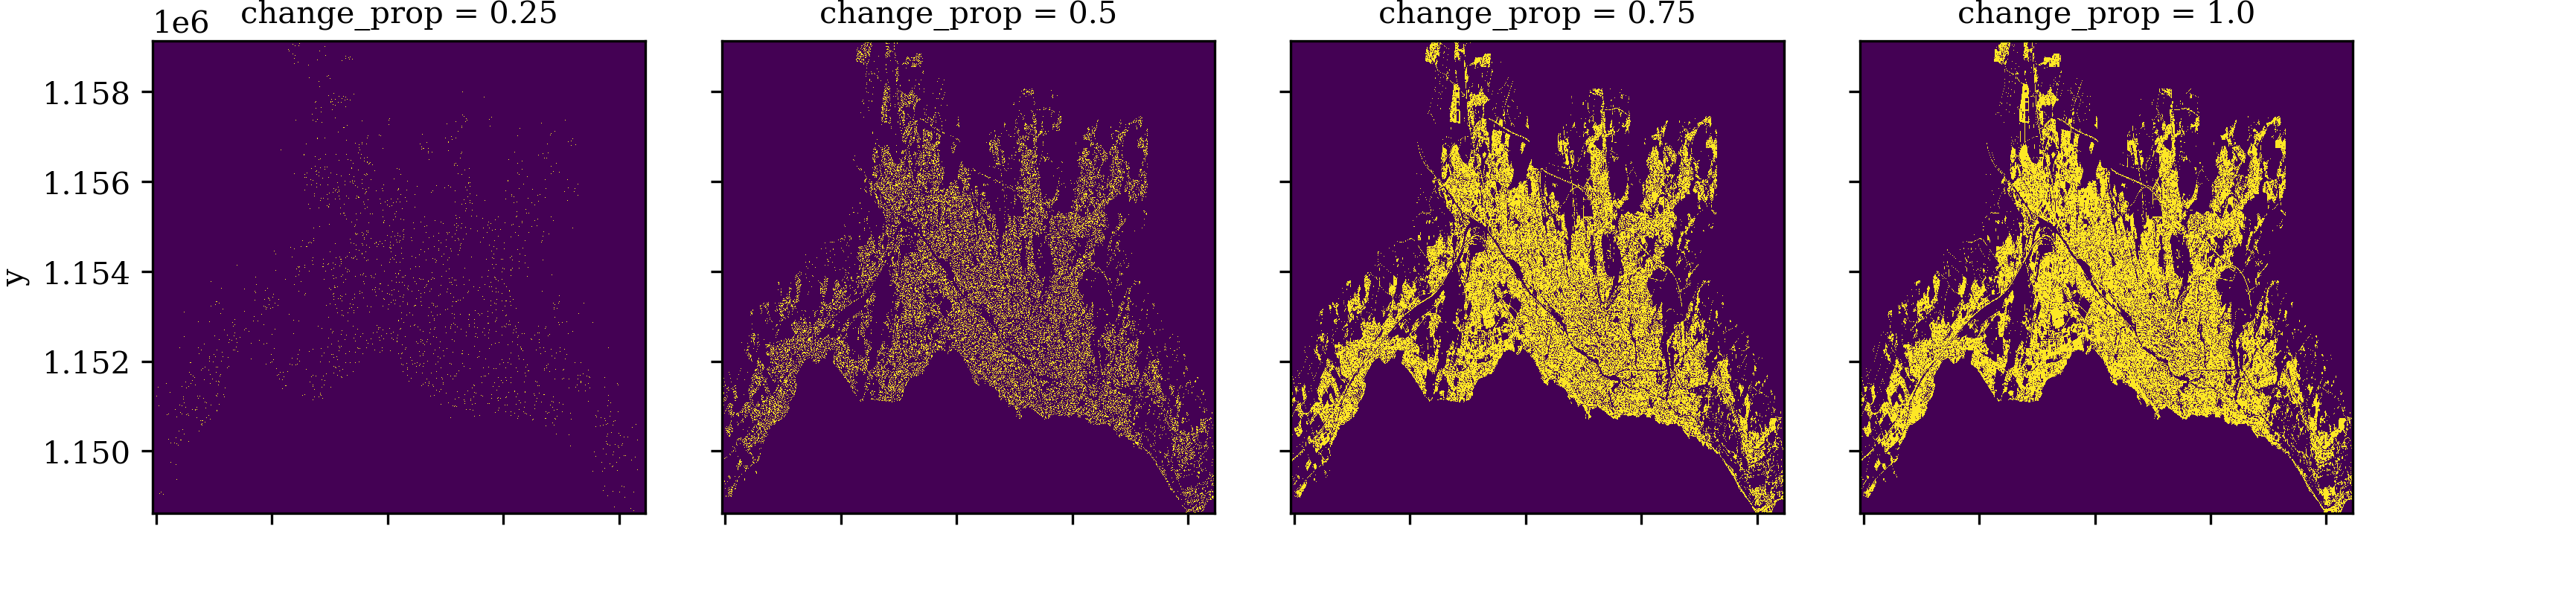
\includegraphics[width=\textwidth]{figures/scenarios-prop-lulc.png}
  \end{subfigure}
  \begin{subfigure}{\textwidth}
    \centering    
    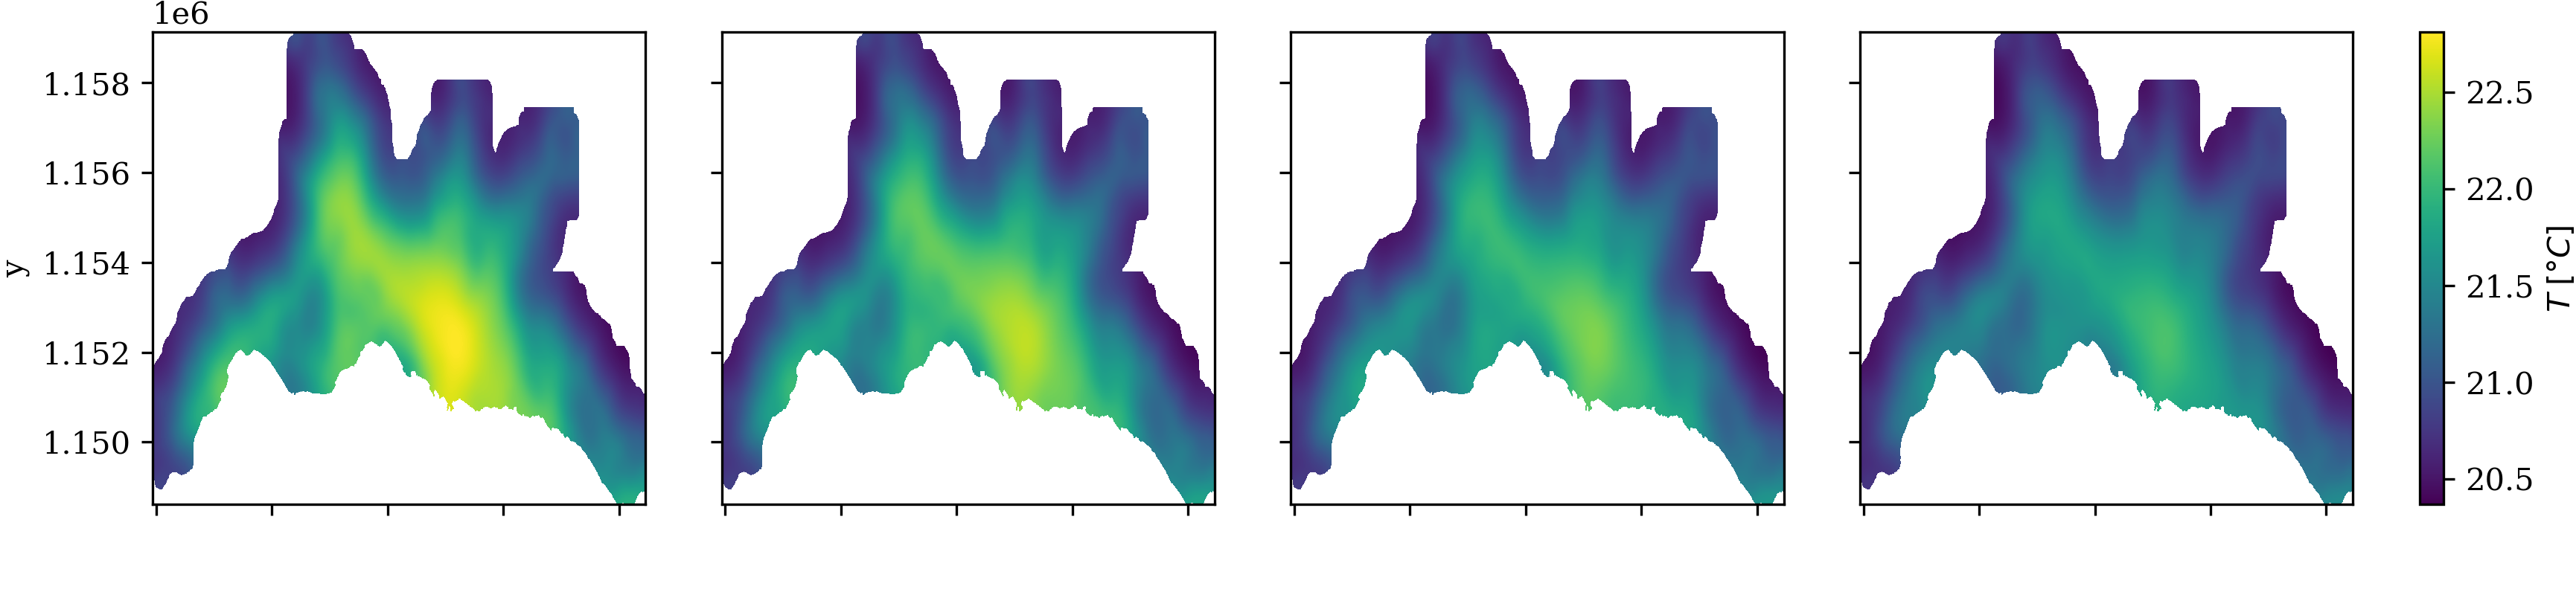
\includegraphics[width=\textwidth]{figures/scenarios-prop-T.png}  
  \end{subfigure}
  \begin{subfigure}{\textwidth}
    \centering    
    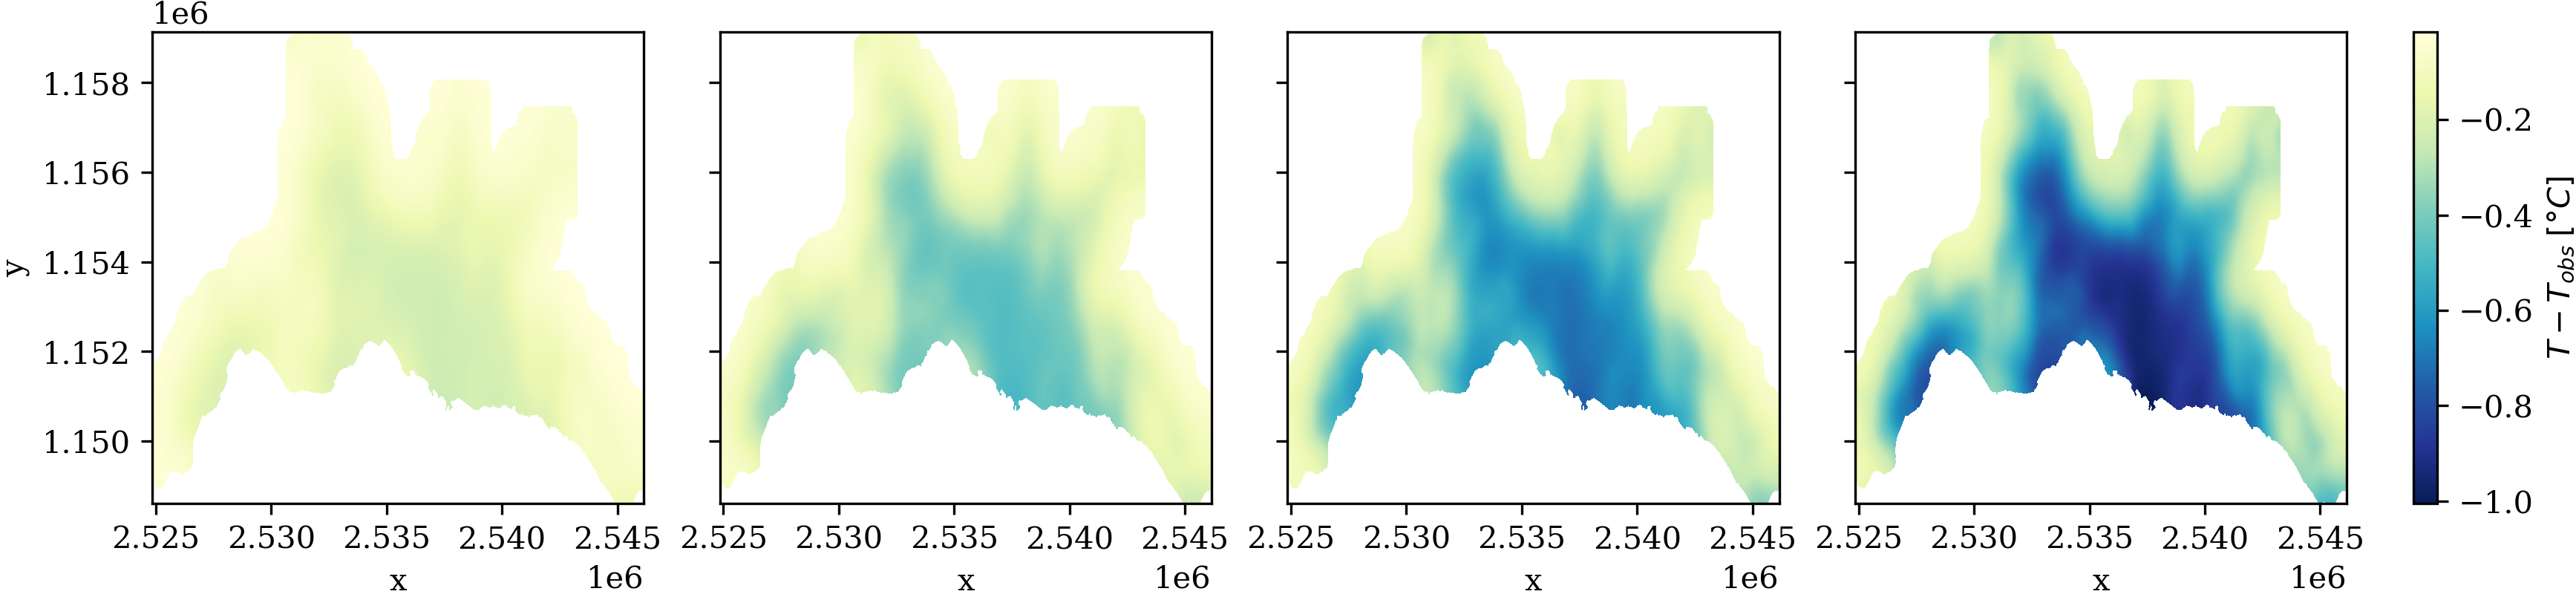
\includegraphics[width=\textwidth]{figures/scenarios-prop-mitigation.png}
  \end{subfigure}
  \caption{\label{fig:scenarios-prop} Scenario raster maps with an increasing (from left to right) proportion of the pixels changed to its corresponding LULC code with high tree canopy cover. The rows respectively feature the pixels where the LULC is changed (top), the simulated air temperature (middle) and the simulated heat mitigation (bottom).}
\end{figure}





\subsection{Effect of the spatial configuration of tree cover}

The relationships between the landscape metrics computed for each scenario sample and the corresponding average simulated temperature are displayed in \autoref{fig:scenarios-config} (see \ref{sec:effect-config}).

\begin{figure}
  \centering
  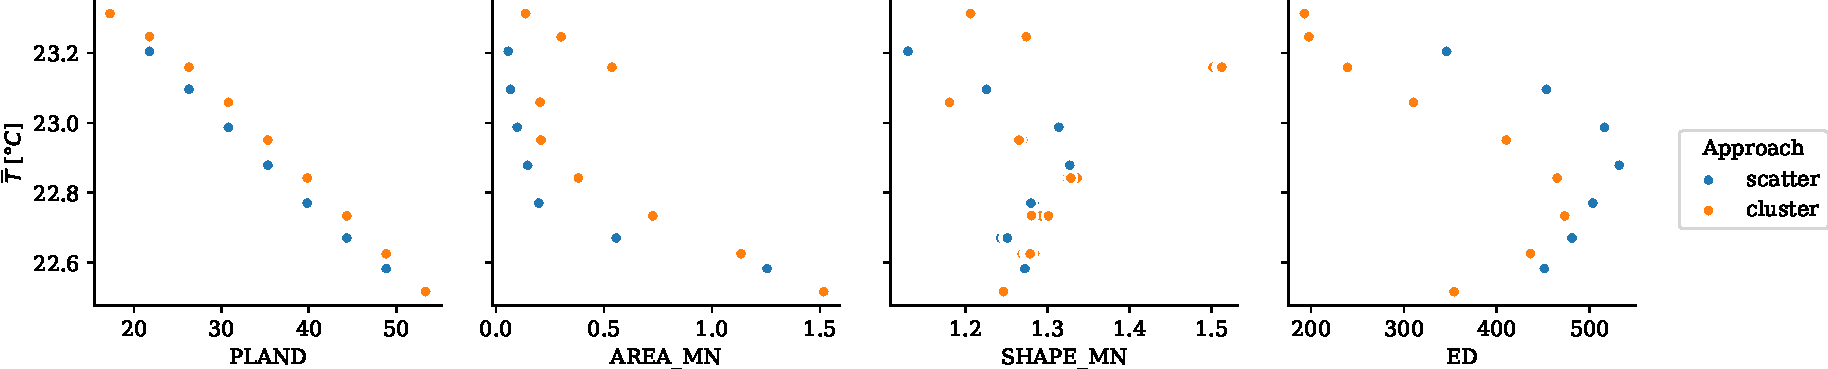
\includegraphics[width=\textwidth]{figures/scenarios-config}
  \caption{\label{fig:scenarios-config} Relationship between landscape metrics and the average simulated temperature $\overline{T}$ for each scenario sample, colored to distinguish scenarios simulated with the ``cluster'' and ``scatter'' approaches.}
\end{figure}

\subsection{Effects on human exposure}

% The fraction of the population exposed to temperatures higher than certain thresholds for a set of scenarios with increasing proportion of tree cover
The relationship between human exposure to higher air temperatures and the proportion of tree cover is shown in \autoref{fig:human-exposure} (see \ref{sec:human-exposure}).

\begin{figure}[ht]
  \centering
  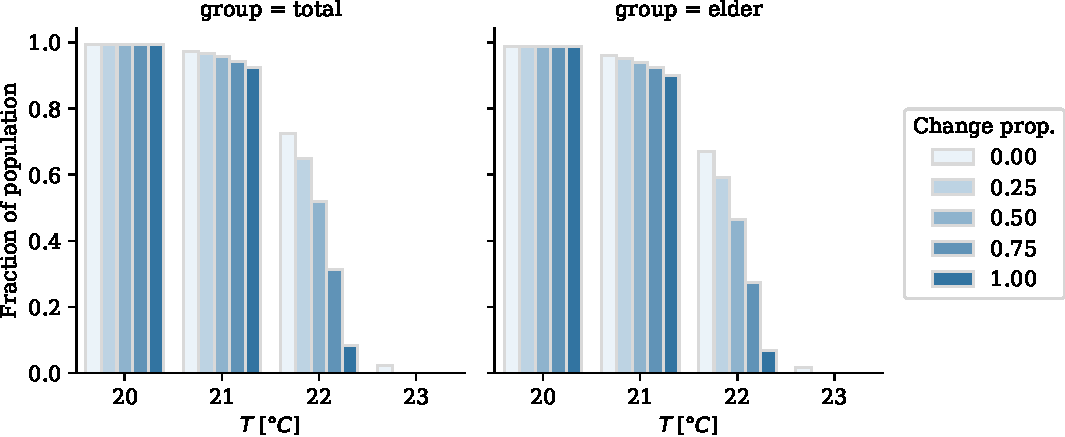
\includegraphics[width=\textwidth]{figures/human-exposure}
  \caption{\label{fig:human-exposure} Fraction of the population exposed to higher temperatures than 20, 21, 22 and 23 $\degree$C respectively, for an increasing proportion of pixel pixels changed to its corresponding LULC code with high tree canopy cover.}
\end{figure}


\section{Discussion}



\section{Conclusion}


\appendix

\section{Biophysical table}
\label{sec:biophysical-table}

% Biophysical table (before the reclassification), as comma-separated values (CSV).
% \url{https://github.com/martibosch/lausanne-heat-islands/blob/master/data/raw/biophysical-table.csv}
The biophysical table for the LULC codes (before the reclassification) is shown in \autoref{tab:biophysical-table}. The crop and water coefficients are based on Allen et al. \cite{allen1998crop}, while rock, soil and urban coefficients are derived from the results of Grimmond and Oke \cite{grimmond1999evapotranspiration} in the city of Chicago. Given that the evapotranspiration of the vegetation and crops is subject to seasonal changes in temperate zones such as Switzerland \cite{allen1998crop}, the values that correspond to the mid-season estimation (June to August) in \cite{nistor2016mapping}.
The albedo values are based on the work of Steward et al. \cite{stewart2012local}.
The shade column, which represents the proportion of tree cover of each LULC class, is computed after the reclassification procedure described in \autoref{sec:refin-lulc-class}.

\begin{table}[!h]
  % \begin{adjustwidth}{-.02\textwidth}{0cm}
    \caption{\label{tab:biophysical-table} Biophysical table (before the reclassification). The source comma-separated value (CSV) file used in the computational workflow is available at \url{https://github.com/martibosch/lausanne-heat-islands/blob/master/data/raw/biophysical-table.csv}.}
    \begin{center}
      \begin{tabular}{ c p{.28\textwidth} p{.16\textwidth} c c c }
        \toprule
        LULC code & Description & Case & $K_c$ & Albedo & Green area \\
        \midrule
        0 & building & artificial & 0.4 & 0.1-0.25 & 0 \\ % 0.142
        1 & road, path & artificial & 0.35 & 0.15 & 0 \\ % 0.141
        2 & sidewalk & artificial & 0.35 & 0.15 & 0 \\
        3 & traffic island & artificial & 0.35 & 0.15 & 0 \\
        4 & rail & artificial & 0.35 & 0.15 & 0 \\
        5 & airfield & artificial & 0.4 & 0.2 & 0 \\
        6 & pond & water & 0.45 & 0.15 & 0 \\
        7 & other impervious & artificial & 0.36 & 0.15 & 0 \\
        8 & field, meadow, pasture & vegetation & 0.9 & 0.2 & 1 \\
        9 & vineyards & vegetation & 0.7 & 0.2 & 1 \\
        10 & other intensive farming & vegetation & 1.05 & 0.2 & 1 \\
        11 & garden & artificial & 0.32 & 0.2 & 1 \\
        12 & wetland & water & 0.45 & 0.1 & 1 \\
        13 & other green & vegetation & 0.45 & 0.2 & 1 \\
        14 & backwater & water & 0.65 & 0.05 & 1 \\
        15 & water course & water & 0.65 & 0.05 & 0\\
        16 & reed & water & 0.45 & 0.1 & 1\\
        17 & dense forest & vegetation & 1.5 & 0.15 & 1 \\
        18 & densely wooded pasture & vegetation & 1.15 & 0.15 & 1 \\
        19 & open wooded pasture & vegetation & 1.15 & 0.2 & 1 \\
        20 & other wooded & vegetation & 1.15 & 0.15 & 1\\
        21 & bare rocks & rock and soil & 0.2 & 0.25 & 0 \\
        22 & glacier & water & 0.52 & 0.1 & 0 \\
        23 & sand & rock and soil & 0.3 & 0.25 & 0 \\
        24 & gravel pit & artificial & 0.36 & 0.25 & 0 \\
        25 & other non-vegetated & artificial & 0.36 & 0.15 & 0 \\
        \bottomrule
      \end{tabular}
      % \caption{\label{tab:evapotranspiration-coefficients}
      % Evapotranspiration coefficients for each LULC class (see \nameref{table-biophysical}). Crop and water coefficients are based on Allen et al. \cite{allen1998crop}, while rock, soil and urban coefficients are derived from the results of Grimmond and Oke \cite{grimmond1999evapotranspiration} in the city of Chicago. Given that the evapotranspiration of the vegetation and crops is subject to seasonal changes in temperate zones such as Switzerland \cite{allen1998crop}, the values that correspond to the mid-season estimation (June to August) in \cite{nistor2016mapping}.
      % The albedo values are based on the work of Steward et al. \cite{stewart2012local}.
      % The source comma-separated value (CSV) file used in the computational workflow is available at \url{https://github.com/martibosch/lausanne-heat-islands/blob/master/data/raw/biophysical-table.csv}.
      % }
    \end{center}
    % \vspace{.5em}
    % \textbf{Table S3.} Biophysical table. The crop and water coefficients are based on Allen et al. \cite{allen1998crop}, while rock, soil and urban coefficients are derived from the results of Grimmond and Oke \cite{grimmond1999evapotranspiration} in the city of Chicago. Given that the evapotranspiration of the vegetation and crops is subject to seasonal changes in temperate zones such as Switzerland \cite{allen1998crop}, the values that correspond to the mid-season estimation (June to August) in \cite{nistor2016mapping}.
    % The albedo values are based on the work of Steward et al. \cite{stewart2012local}.
    % The source comma-separated value (CSV) file used in the computational workflow is available at \url{https://github.com/martibosch/lausanne-heat-islands/blob/master/data/raw/biophysical-table.csv}.
  % \end{adjustwidth}
\end{table}


% \section{Relationships between the spatial patterns of tree canopy and air temperature}
% \label{sec:spatial-relationships}

% Exploration of relationships between the spatial patterns of tree canopy and air temperature, as Jupyter Notebook (IPYNB) \url{https://github.com/martibosch/lausanne-greening-scenarios/blob/master/notebooks/spatial-relationships.ipynb}.

\section{Effect of the proportion of tree cover}
\label{sec:effect-prop}

% The code for the evaluation of scenarios generated to explore the effect of increasing the proportion of tree cover
The code to generate the figures \ref{fig:greening-lulc-change}, \ref{fig:scenarios-prop}, \ref{fig:scenarios-prop-regplot} and \ref{fig:scenarios-prop-hists} is available as a Jupyter Notebook (IPYNB) at \url{https://github.com/martibosch/lausanne-greening-scenarios/blob/master/notebooks/scenarios-prop.ipynb}.

\begin{figure}[ht]
  \centering
  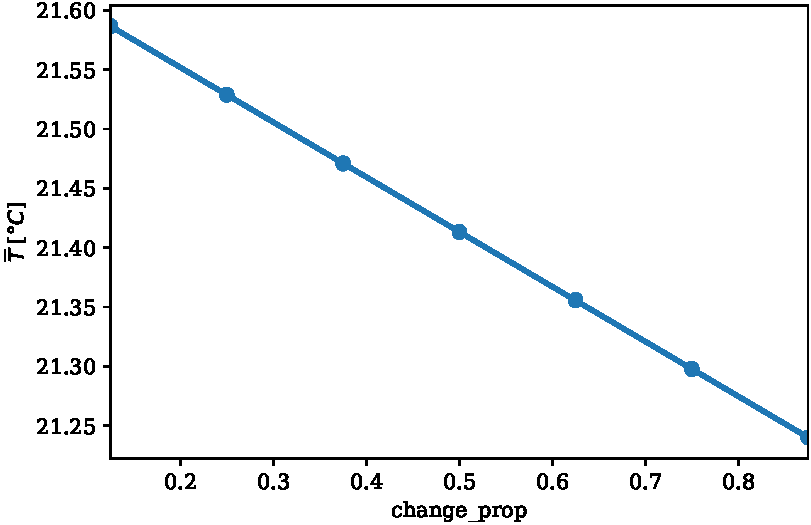
\includegraphics[width=.6\textwidth]{figures/scenarios-prop-regplot}
  \caption{\label{fig:scenarios-prop-regplot}}
\end{figure}


\begin{figure}[ht]
  \centering
  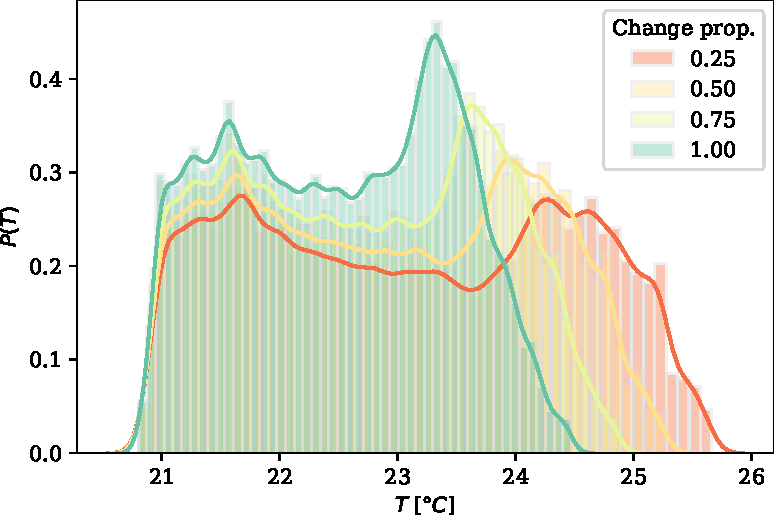
\includegraphics[width=.6\textwidth]{figures/scenarios-prop-hists}
  \caption{\label{fig:scenarios-prop-hists}}
\end{figure}


\section{Effect of the spatial configuration of tree cover}
\label{sec:effect-config}

% Evaluation of scenarios generated to explore the effect of the spatial configuration of tree cover, as Jupyter Notebook (IPYNB) \url{https://github.com/martibosch/lausanne-greening-scenarios/blob/master/notebooks/scenarios-config.ipynb}.
The code to generate \autoref{fig:scenarios-config} is available as a Jupyter Notebook (IPYNB) at \url{https://github.com/martibosch/lausanne-greening-scenarios/blob/master/notebooks/scenarios-config.ipynb}.


\section{Relationship between human exposure to higher air temperatures and the proportion of tree cover}
\label{sec:human-exposure}

% Evaluation of scenarios generated to explore the effect of the spatial configuration of tree cover, as Jupyter Notebook (IPYNB) \url{https://github.com/martibosch/lausanne-greening-scenarios/blob/master/notebooks/human-exposure.ipynb}.

The code to generate \autoref{fig:human-exposure} is available as a Jupyter Notebook (IPYNB) at \url{https://github.com/martibosch/lausanne-greening-scenarios/blob/master/notebooks/human-exposure.ipynb}.


\section*{References}

\bibliography{references}
\bibliographystyle{unsrt}

\end{document}
